%中間審査概要テンプレート ver. 3.0

\documentclass[uplatex,twocolumn,dvipdfmx]{jsarticle}
\usepackage[top=22mm,bottom=22mm,left=22mm,right=22mm]{geometry}
\setlength{\columnsep}{10mm}
\usepackage[T1]{fontenc}
\usepackage{txfonts}
\usepackage[expert,deluxe]{otf}
\usepackage[dvipdfmx,hiresbb]{graphicx}
\usepackage[dvipdfmx]{hyperref}
\usepackage{pxjahyper}
\usepackage{secdot}





%タイトルと学生番号,名前だけ編集すること
\title{\vspace{-5mm}\fontsize{14pt}{0pt}\selectfont  ゲーム攻略Wikiにおけるプロジェクトマネジメント状況の分析}
\author{\normalsize プロジェクトマネジメントコース 矢吹研究室 1342014 泉 雄太}
\date{}
\pagestyle{empty}
\begin{document}
\fontsize{10.5pt}{\baselineskip}\selectfont
\maketitle





%以下が本文
\section{背景}

コンピューターゲームの攻略情報を体系的にまとめたものとして攻略本というものがある.初期の攻略本は小規模のグループが攻略情報をまとめ,同人誌として発行していた.のちにファミリーコンピューターが普及すると商業出版がデータなどをまとめた攻略本を出版しはじめた.インターネットが普及した現代では,ゲームの攻略wikiが登場し,一般消費者が攻略情報を書き込む形のサイトが増えている.
これらの本やサイトは通常,特定あるいは不特定多数の人間が集まって作られている.そのためこれらを作成する過程ではプロジェクトマネジメントが行われているのではないかと考え,本研究ではゲーム攻略wikiを対象にした調査を行う.

また,ゲーム攻略wikiの特性を探るため,同じくwikiを使用している百科事典サイトであるWikipediaとの比較を行う.



\section{目的}

データマイニングにより,ゲーム攻略wikiにおけるプロジェクトマネジメントの状況を分析し,ネット上での不特定多数によるプロジェクトの特性を探る.

\section{手法}

ゲーム攻略wiki内の編集履歴をもとに編集者ID,編集回数,編集文字数を編集者ごとに記録し,Rを用いてヒストグラムを作成する.また,作成したヒストグラムを別の研究で作成された,Wikipediaのヒストグラムと比較する.

\section{想定される成果物}

ゲーム攻略wikiにおける編集回数のヒストグラムおよび編集文字数のヒストグラム.

\section{進捗状況}

2011年発売のプレイステーション3/Xbox360/Windows用ソフト「The Elder Scrolls V Skyrim」の日本語版攻略wiki\cite{wiki}を対象に調査をおこなっている.現在,同wikiのページのうち3ページ分の調査を行い,106人の編集者の編集回数と編集文字数を記録し,それらのデータをもとにヒストグラムを作成した.



%図の挿入
\begin{figure}[thbp]
 \begin{minipage}{1\hsize}
  \begin{center}
   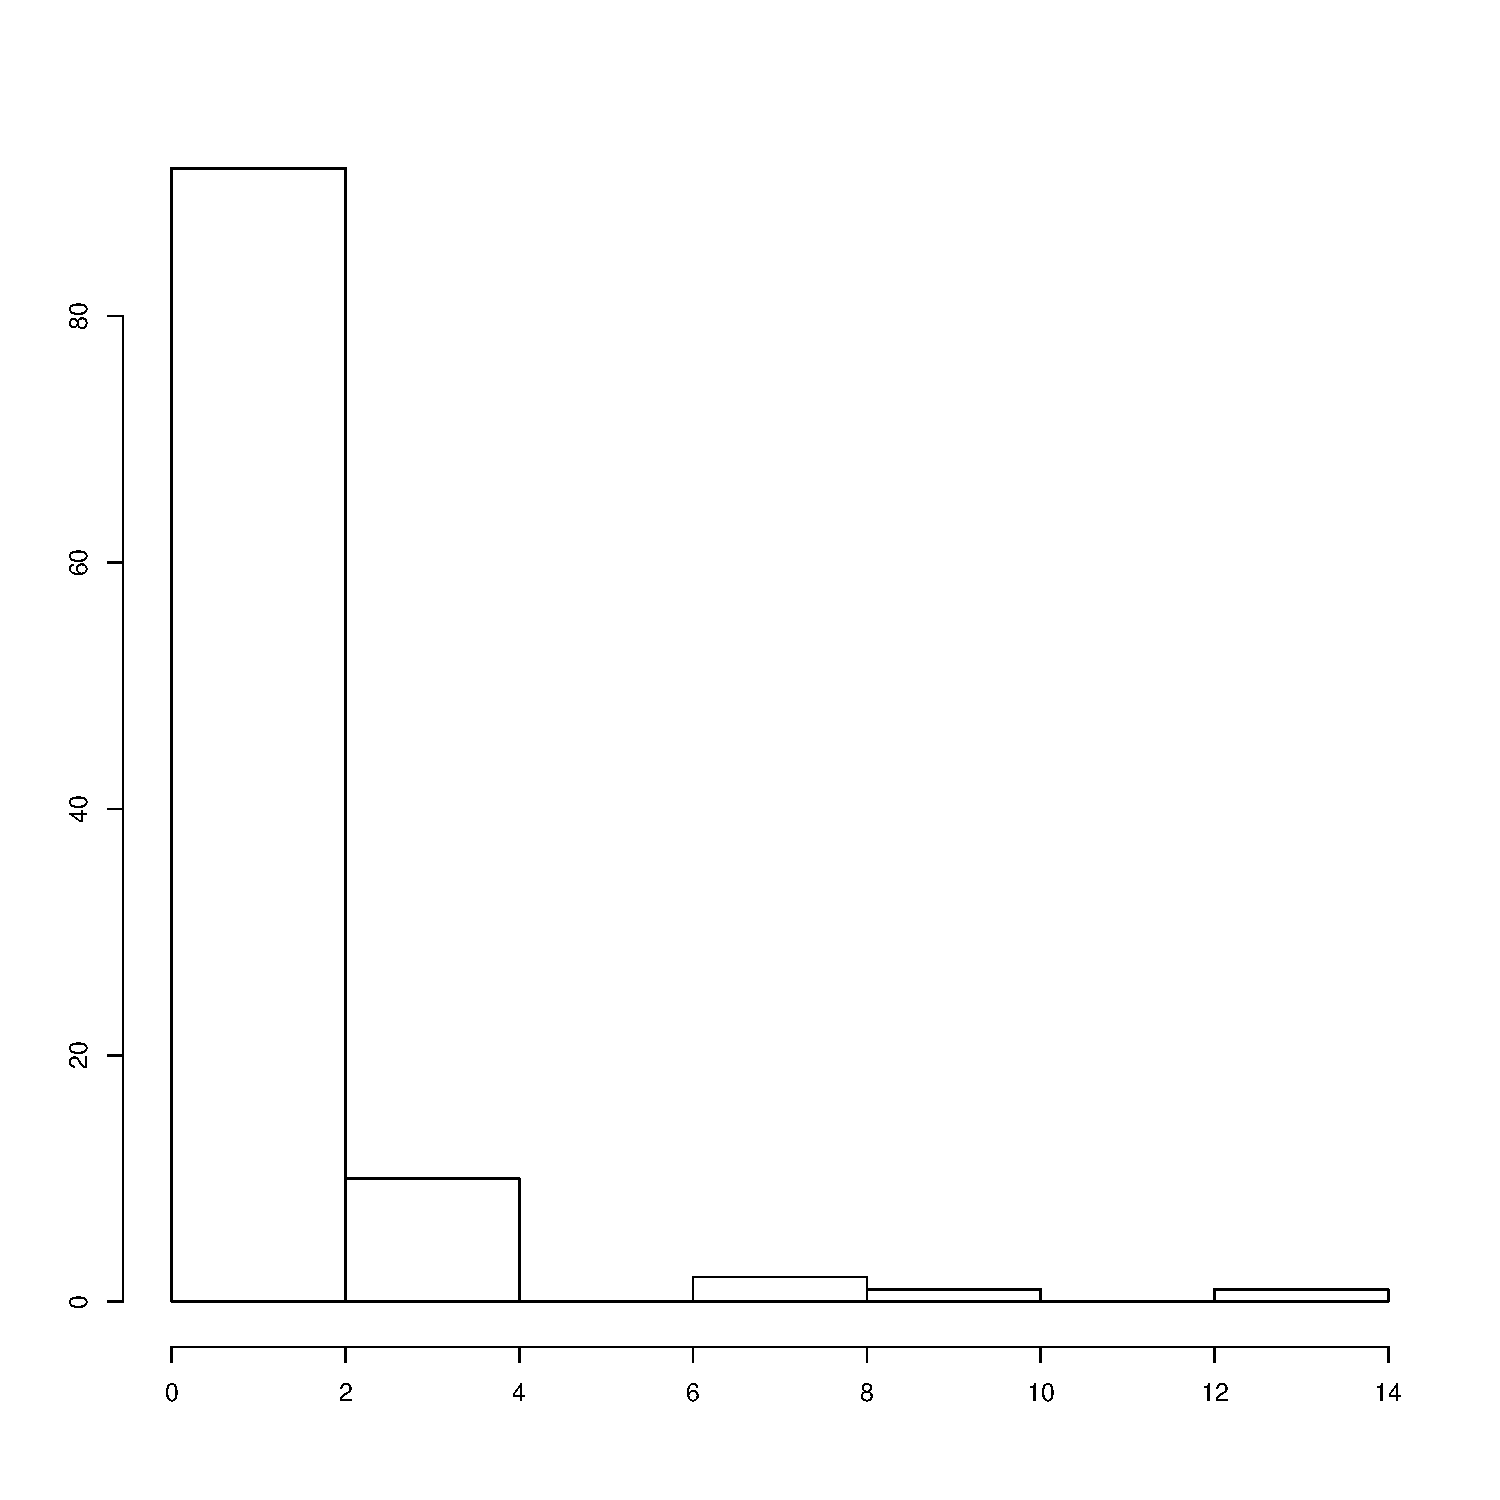
\includegraphics[width=60mm]{skyrmK.pdf}
   \caption{編集回数のヒストグラム}
   \label{left}
  \end{center}
 \end{minipage}\\
 \begin{minipage}{1\hsize}
  \begin{center}
   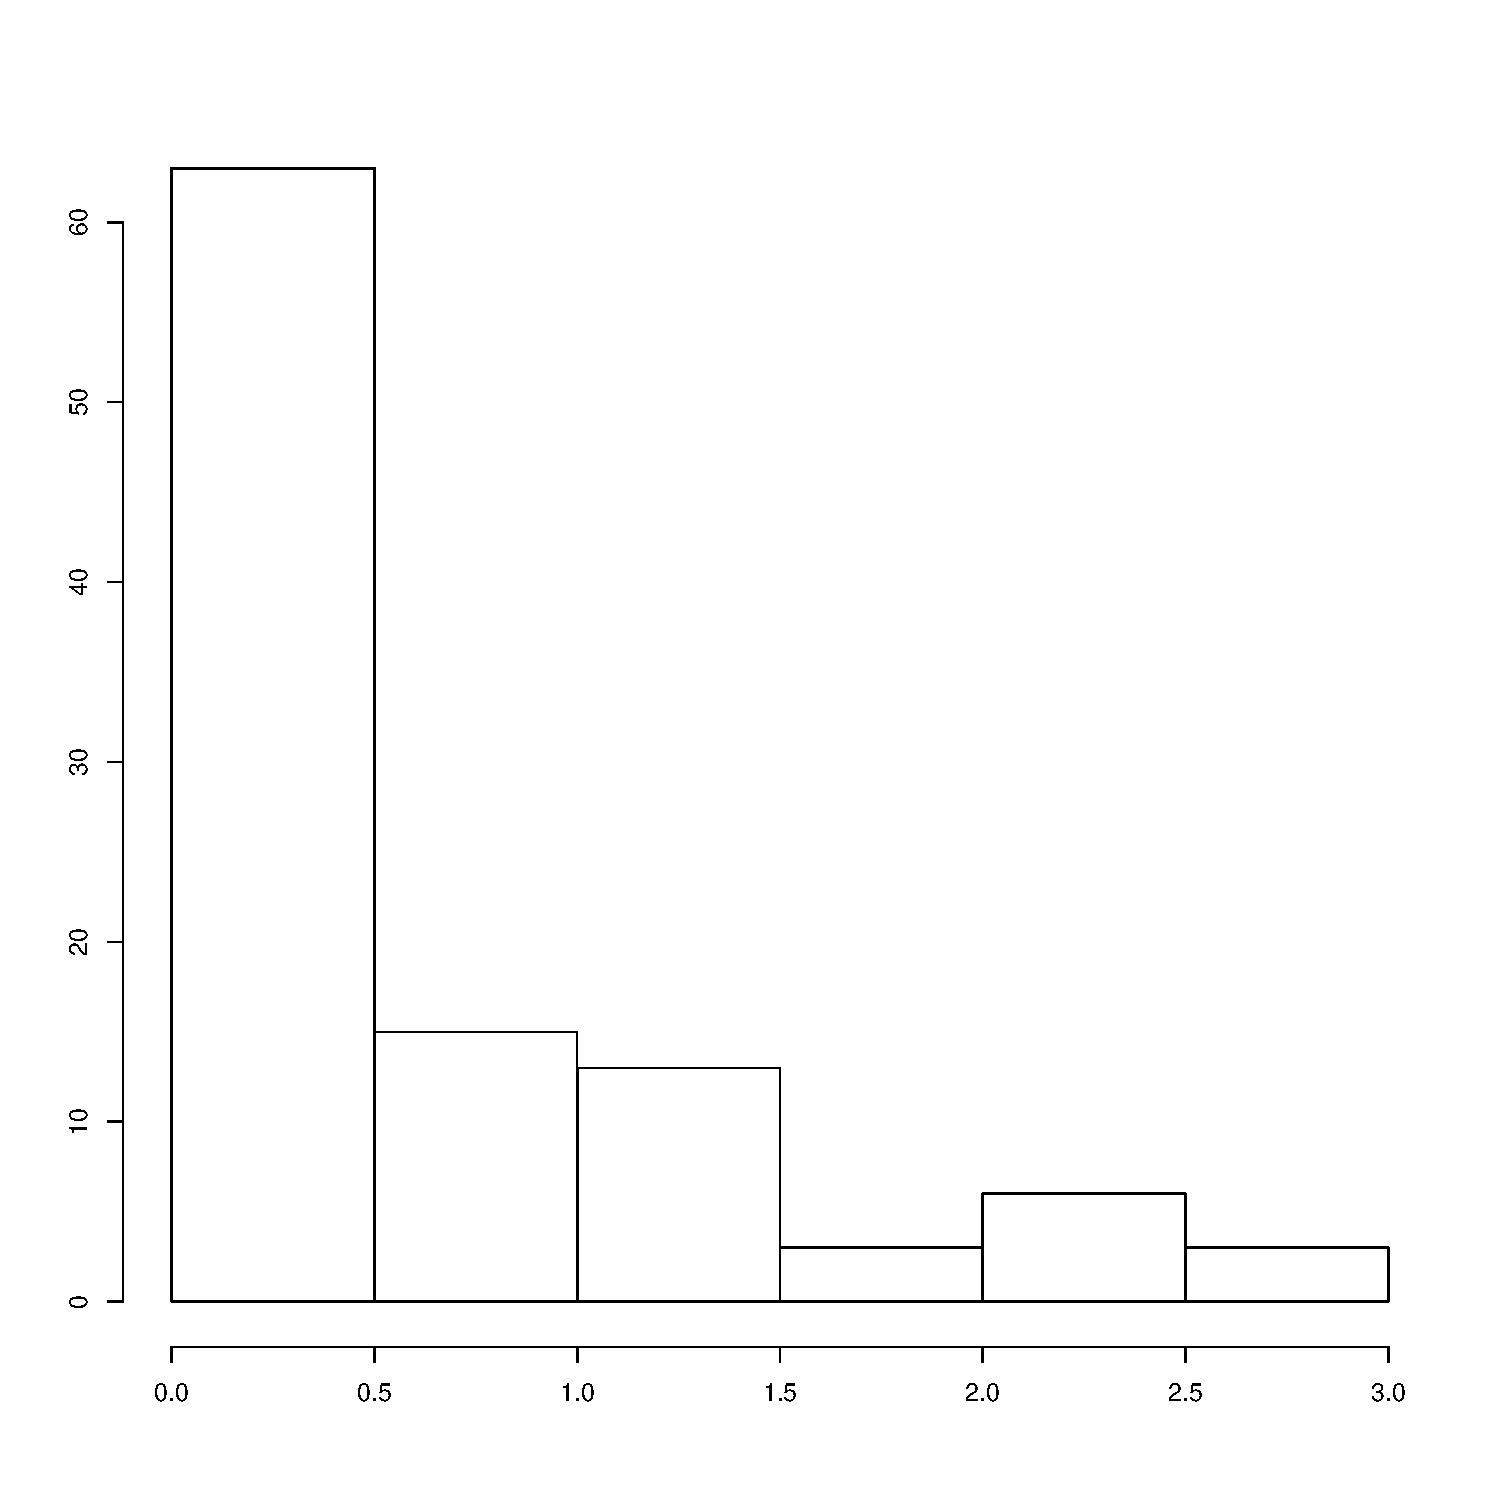
\includegraphics[width=60mm]{skyrmG.pdf}
   \caption{編集文字数のヒストグラム}
   \label{right}
  \end{center}
 \end{minipage}
\end{figure}


\section{今後の計画}

wikiからデータを取得する工程を自動化するために,pukiwikiから機械的にデータを取得する方法を見つける.

\bibliographystyle{junsrt}
\bibliography{biblio}%「biblio.bib」というファイルが必要.

\end{document}
